\documentclass[10pt,a4paper,twocolumn]{article}
\usepackage[utf8]{inputenc}
\usepackage[T1]{fontenc}
\usepackage{graphicx}
\graphicspath{{./figures/}}
\usepackage{amsmath}
\usepackage{amsfonts}
\usepackage{amssymb}
\usepackage[left=1.5cm, right=1.5cm, top=2.50cm, bottom=2.50cm]{geometry}
\usepackage{multicol}
\usepackage{float}

\author{Fabian Schubert}
\title{Nonlinear Dendritic Coincidence Detection for Supervised Learning}

\usepackage{natbib}
\bibliographystyle{apalike}

\renewcommand{\arraystretch}{1.5}

\begin{document}
	\maketitle

		\section{Introduction}
		
		In recent years, a growing body of research has addressed the 
		functional implications of the distinct physiology and anatomy of 
		cortical pyramidal neurons. In particular, on the theoretical side,
		we saw a paradigm shift from treating neurons as point-like electrical
		structures towards embracing the entire dendritic structure. This was 
		mostly due to the fact that experimental work uncovered dynamical properties
		of these cells that simply could not be accounted for by point models.
		
		An important finding was that the apical dendritic tree of
		cortical pyramidal neurons can act as a separate nonlinear synaptic 
		integration zone. Under certain conditions, a dendritic $\rm Ca^{2+}$ spike
		can be elicited that propagates towards the soma, causing rapid, bursting
		spiking activity. One of the cases in which dendritic spiking can occur
		was termed 'backpropagation-activated $\rm Ca^{2+}$ spike firing' 
		('BAC firing'): A single somatic spike can backpropagate towards the apical
		spike initiation zone, in turn significantly facilitating the initiation of 
		a dendritic spike. This reciprocal coupling is believed to act as a form of
		coincidence detection: If apical and basal synaptic input co-occurs, the 
		neuron can respond with a rapid burst of spiking activity. The firing rate
		of these temporal bursts exceeds the firing rate that is maximally achievable 
		under basal synaptic input alone, thus representing a form of temporal coincidence
		detection between apical and basal input.
		
		Naturally, these mechanisms also affect plasticity and thus learning
		within the cortex. While the interplay between basal and apical stimulation and
		its effect on synaptic efficacies is subject to ongoing research, there is
		some evidence that BAC-firing tends to shift plasticity towards long-term potentiation
		(LTP). Thus, coincidence between basal and apical input appears to also gate synaptic
		plasticity.
		
		In our work, we combined a phenomenological model predicting the output
		firing rate as a function of two streams of synaptic input (subsuming basal and apical input)
		with a BCM-like plasticity rule on basal synapses. LTP was induced in our model 
		if the postsynaptic activity surpassed a threshold level that was only achievable if 
		both basal and apical inputs were present. Therefore, we hypothesized that 
		this combination of neural activation and plasticity rules would lead to an
		increased correlation between basal and apical input.
		
		Furthermore, this temporal alignment could potentially facilitate apical inputs to act
		as top-down teaching signals, without the need for an explicit error-driven
		learning rule. Thus, we also tested our model in a simple linear 
		supervised classification task and compared it to the performance of simple
		point neuron combined with a BCM-plasticity rule on the basal inputs.
		
		\section{Model}
		
		\subsection{Neuron Model}
		
		The neuron model used throughout this study is a discrete-time rate encoding model that
		uses two separate input variables, subsuming the total synaptic
		input current injected arriving at the basal (proximal) and apical (distal) 
		dendritic structure of a pyramidal neuron, respectively. The model is a slightly
		simplified version of a phenomenological model proposed by \citet{Shai_2015}.
		Denoting the input currents by $I_p$ (proximal) and $I_d$ (distal), 
		the model is written as
		%%%%%%%%%%%%%%%%%%%%%%%%%%%%%%%%%%%%%
		\begin{align}
		\begin{split}
		y\left(t\right) &= \sigma\left( I_p(t) - \theta_{p0} \right)
		\left[1-\sigma\left(I_d(t) - \theta_d\right)\right] \\
		&+ \alpha \sigma\left(I_d(t) - \theta_d \right)\sigma\left( I_p(t) - \theta_{p1} \right)
		\end{split} \label{eq:comp_model}\\
		\sigma(x) &\equiv \frac{1}{1+\exp(-4x)} \; .
		\end{align}
		%%%%%%%%%%%%%%%%%%%%%%%%%%%%%%%%%%%%%
		Here, $\theta_{p0}$, $\theta_{p1}$ and $\theta_d$ are threshold variables with
		respect to proximal and distal input. Overall, this equation describes two distinct
		regions of neural activation in the $(I_p, I_d)$-space which differ in their
		maximal firing rates, which are set to $1$ and $\alpha$, where $0 < \alpha < 1$.
		A plot of \eqref{eq:comp_model} is shown in Fig.~\ref{fig:comp_model}.
		%%%%%%%%%%%%%%%%%%%%%%%%%%%%%%%%%%%%%
		\begin{figure}
			\centering
			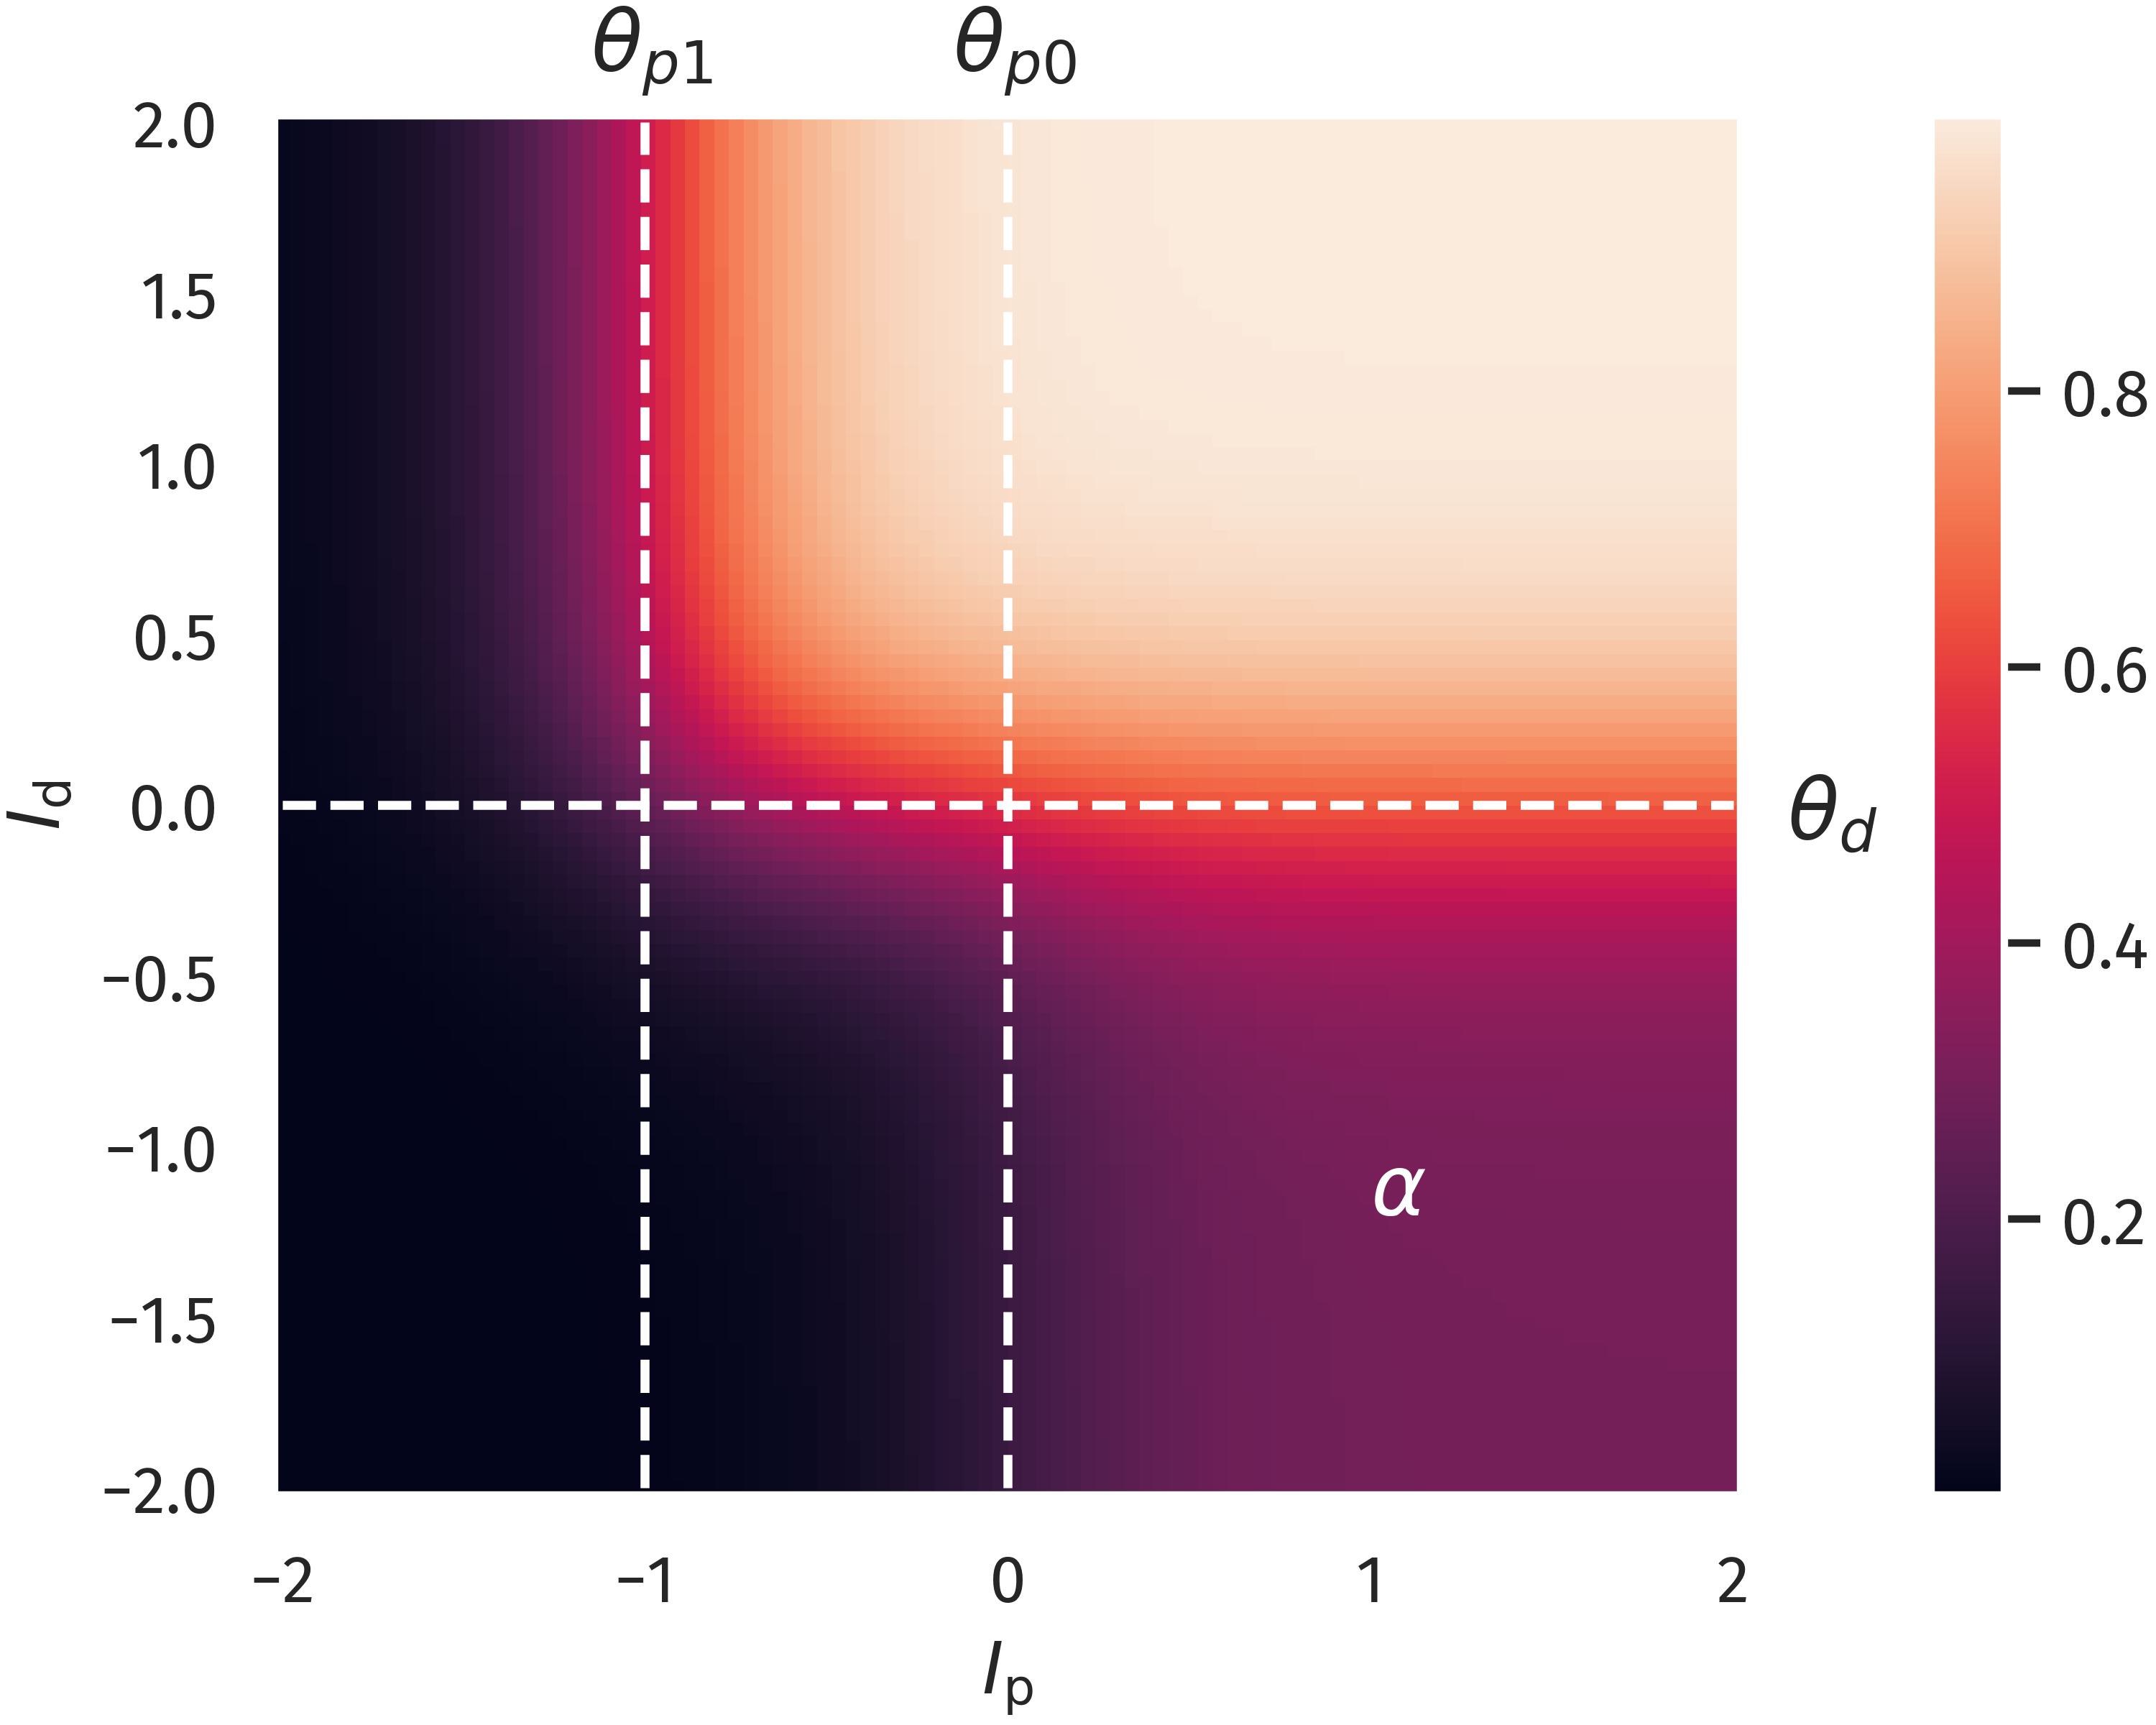
\includegraphics[width=0.8\columnwidth]{plot_comp_mod_marks.png}
			\caption{{\bf Two-compartment rate model.} Firing rate as a
			function of proximal and distal input $I_p$ and $I_d$, 
			see \eqref{eq:comp_model}. 
			The thresholds $\theta_{p0}$, $\theta_{p1}$ and $\theta_d$ define
			two regions of neural activity with a a maximal firing rate of $1$
			and $\alpha$.}
			\label{fig:comp_model}
		\end{figure}
		%%%%%%%%%%%%%%%%%%%%%%%%%%%%%%%%%%%%%
		
		In all our numerical experiments, we compared this model with a 
		simple point neuron model that was given by
		%%%%%%%%%%%%%%%%%%%%%%%%%%%%%%%%%%%%%
		\begin{equation}
			y(t) = \sigma\left(I_p(t) + I_d(t) - \theta \right) \; .
		\end{equation}
		%%%%%%%%%%%%%%%%%%%%%%%%%%%%%%%%%%%%%
		In all our numerical experiments, the apical input $I_d$ was generated
		``as is", meaning, it was not dynamically calculated as a superposition
		of multiple presynaptic inputs, but given by
		%%%%%%%%%%%%%%%%%%%%%%%%%%%%%%%%%%%%%
		\begin{equation}
			I_d(t) = n_d(t) x_d(t) - b_d(t) \; ,
			\label{eq:I_d}
		\end{equation}
		%%%%%%%%%%%%%%%%%%%%%%%%%%%%%%%%%%%%%
		where $n_d(t)$ is a scaling factor, $x_d(t)$ a pre-generated
		discrete time sequence and $b_d(t)$ a bias. Note that $n_d$ and $b_d$ 
		are time dependent since they were subject to adaptation processes 
		that are described in the next section.
		
		Similarly, $I_p(t)$ was given by
		%%%%%%%%%%%%%%%%%%%%%%%%%%%%%%%%%%%%%
		\begin{equation}
			I_p(t) = n_p(t) \sum_{i=1}^{N} x_{p,i}(t) w_i(t) - b_p(t) \; ,
		\end{equation}
		%%%%%%%%%%%%%%%%%%%%%%%%%%%%%%%%%%%%%
		where $N$ is the number of presynaptic afferents, $x_{p,i}(t)$ the
		corresponding sequences and $w_i(t)$ the synaptic efficacies.
		As for $I_d(t)$, $n_p(t)$ and $b_p(t)$ was used as a time dependent
		scaling and bias.
		
		\subsection{Plasticity}
		
		We implemented a BCM-like plasticity rule for the basal 
		synaptic weights given by the following update equation:
		%%%%%%%%%%%%%%%%%%%%%%%%%%%%%%%%%%%%%
		\begin{equation}
			w_i(t+1) = w_i(t) + \mu_w (x_{p,i}(t) - \langle x_{p,i}\rangle_t)
			y(t)\left[y(t) - \theta_y \right]
			\label{eq:bcm_plast}
		\end{equation}
		%%%%%%%%%%%%%%%%%%%%%%%%%%%%%%%%%%%%%
		While the classical BCM-rule dynamically modifies the 
		threshold $\theta_y$ to stabilize weights, we used a
		synaptic normalization constraint
		%%%%%%%%%%%%%%%%%%%%%%%%%%%%%%%%%%%%%
		\begin{equation}
			w_i(t) \rightarrow \frac{w_i(t)}{\lVert \mathbf{w}(t)\rVert}
		\end{equation}
		%%%%%%%%%%%%%%%%%%%%%%%%%%%%%%%%%%%%%
		in each time step, where $\lVert \mathbf{w}(t)\rVert$ denotes the Euclidean
		norm of the synaptic weight vector. The threshold $\theta_y$ was
		chosen such that LTP is present if neural activity is in the
		high-activity regime (yellow area in Fig.~\ref{fig:comp_model}), while
		LTD is present in the low-activity regime 
		(given by $\alpha$, see Fig.~\ref{fig:comp_model}). Hence, we chose
		$\theta_y = (1+\alpha)/2$.
		
		For comparative reasons, the point neuron model was equipped with the
		same plasticity rule for the proximal weights as \eqref{eq:bcm_plast}, 
		except that the threshold $\theta_y$ was dynamically adjusted as
		%%%%%%%%%%%%%%%%%%%%%%%%%%%%%%%%%%%%%
		\begin{equation}
			\theta_y(t+1) = \left(1-\mu_{av}\right)\theta_y(t) + \mu_{av} y^2(t) \; , 
		\end{equation}
		%%%%%%%%%%%%%%%%%%%%%%%%%%%%%%%%%%%%%
		which is an implementation of a running average of the square activity,
		as used in the classic BCM-rule.
		
		Additionally, the scaling and bias variables were changing dynamically
		according to the following homeostatic plasticity rules:
		%%%%%%%%%%%%%%%%%%%%%%%%%%%%%%%%%%%%%
		\begin{align}
			b_p(t+1) &= b_p(t) + \mu_b \left[I_p(t) - I_p^t\right] \\
			b_d(t+1) &= b_d(t) + \mu_b \left[I_d(t) - I_d^t\right] \\
			n_p(t+1) &= n_p(t) + \mu_n \left[V_p^t - \left( I_p(t) - \tilde{I}_p(t)\right)^2\right] \\
			n_d(t+1) &= n_d(t) + \mu_n \left[V_d^t - \left( I_d(t) - \tilde{I}_d(t)\right)^2\right] \\
			\tilde{I}_p(t) &= (1-\mu_{av})\tilde{I}_p(t-1) + \mu_{av} I_p(t) \\
			\tilde{I}_d(t) &= (1-\mu_{av})\tilde{I}_d(t-1) + \mu_{av} I_d(t)
		\end{align}
		%%%%%%%%%%%%%%%%%%%%%%%%%%%%%%%%%%%%%
		Here, $I_p^t$, $I_d^t$, $V_p^t$ and $V_p^t$ define targets for the 
		temporal means and variances of $I_p$ and $I_d$. The dynamic variables 
		$\tilde{I}_p$ and $\tilde{I}_d$ are simply low-pass filtered running 
		averages of $I_p$ and $I_d$.
		
		A list of all parameter values is given in Table~\ref{tab:parameters}.
		
		%%%%%%%%%%%%%%%%%%%%%%%%%%%%%%%%%%%%%
		\begin{table}
			\begin{tabular}{ l | l || l | l }
				$\theta_{p0}$ & $0$ & $V_d^t$ & $0.25$ \\
				$\theta_{p1}$ & $-1$ & $\mu_b$ & $10^{-3}$ \\ 
				$\theta_{d}$ & $0$ & $\mu_n$ & $10^{-4}$ \\  
				$\alpha$ & $0.3$ & $\mu_{av}$ & $5 \cdot 10^{-3}$ \\   
				$\mu_w$ & $5 \cdot 10^{-5}$ & $I_p^t$ & $0$ \\
				$V_p^t$ & $0.25$ & $I_d^t$ & $0$  
			\end{tabular}
		\caption{Model parameters}
		\label{tab:parameters}
		\end{table}
		%%%%%%%%%%%%%%%%%%%%%%%%%%%%%%%%%%%%%
		
		\section{Results}
		
		In a supervised learning scheme, where the top down input
		arriving at the apical compartment acts as the teaching signal,
		the most straight-forward learning rule for the basal synaptic
		weights would be derived from an appropriate loss function,
		such as a mean square error, based on the difference between 
		basal and apical input, i.e. $I_p - I_d$. Theoretical work has 
		investigated possible learning mechanisms
		that could utilize an intracellular error signal
		\citep{Urbanczik_2014,Schiess_2016,Guerguiev_2017}.
		However, a clear experimental
		evidence for a physical quantity encoding such an error 
		is---to our knowledge---yet to be found.
		
		
		
		
		\bibliography{Dendritic_Learning}
		
\end{document}